\subsection{Создание интегированной библиотеки электронных компонентов в системе Eagle} 
Не смотря на обширный перечень готовых библиотек компонентов, входящих в соствам Eagle, а
так же библиотек, разработанных сообществом пользователей системы, рано или поздно возникает
ситуация, когда готового компонента не существует или существующие компоненты не могут
быть использованы по какой-либо причине.


В процессе разработки <<Универсального устройства терморегулирования на базе микроконтроллера
AVR семейства XMega>> мне потребовался символ и посадочное место для
жидкокристаллического индикатора DST2001PH Rev.B, используемого в устройстве управления.
Так же в стандартной библиотеке Eagle отсутствует символ oбозначающий резистов 0.125 Вт.

Для создания пользовательской библиотеки компонент необходимо из главного меню Eagle
выбрать пункт ''New library''.
\begin{figure}[h]
	\center{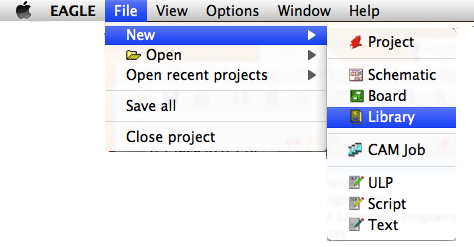
\includegraphics[bb=0 0 474 247, clip, scale=1.0]{new_library.png}}
	\caption{Создание новой библиотеки в системе Eagle}
	\label{img:newLibrary}
\end{figure}
После того как библиотека создана, её необходимо сохранить.


Библиотеки в Eagle состоят из набора:
\begin{itemize}
	\item{} символов;
	\item{} посадочных мест;
	\item{} устройств --- элементов, сопоставляющих схемотическое обозначение
		с посадочным местом.
\end{itemize}

\subsubsection{Создание символа ''DST2001PH''}

Для того, что бы создать новый символ необходимо в меню ''Library'' выбрать пункт ''Symbol...''.
\begin{figure}[h]
	\center{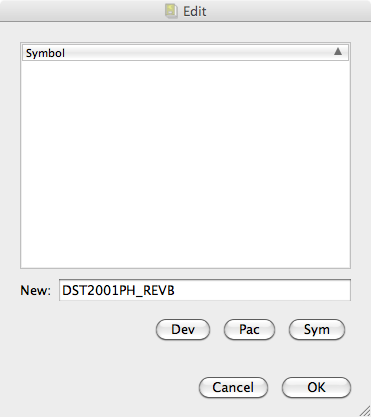
\includegraphics[bb=0 0 371 417, clip, scale=1.0]{new_symbol.png}}
	\caption{Создание нового символа в системе Eagle}
	\label{img:newSymbol}
\end{figure}
После чего ввести название создаваемого символа и нажать кнопку ''Ok''.

В окне редактора символов (рис. \ref{img:symbol}), используя инструменты рисования
Rect, Line, Circle и Arc на соответствующих слоях необходимо нарисовать схемотическое
обозначение элемента.
\begin{figure}[h]
	\center{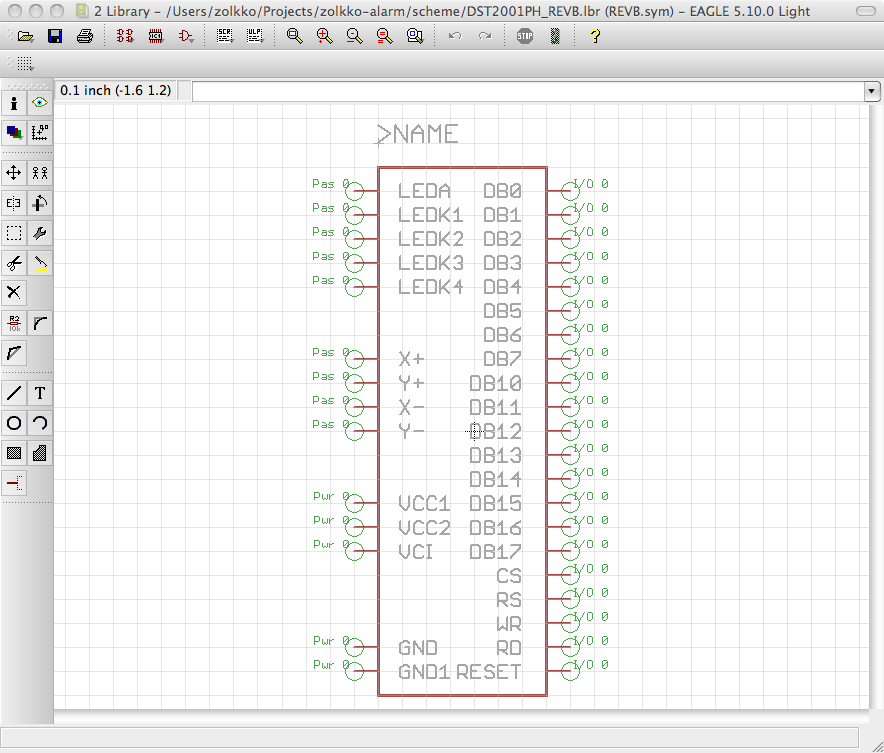
\includegraphics[bb=0 0 884 753, clip, scale=0.5]{symbol.png}}
	\caption{Редактор симоволов в системе Eagle}
	\label{img:symbol}
\end{figure}
Для того, что бы у будущего устройства при его размещении в окне редактора принципиальной
схемы отображалось имя, необходимо используя иструмент ''Text'' на слое ''Names'' ввести
тег ''>NAME''.

Тег ''>VALUE'' будет замещаться на значение элемента, такое как значение
сопротивления резистора. Так как необходимости в выводе значения для симола DST2001PH нет,
то производить ввод этого текста в редакторе симолов не нужно.

Следующим шагом при создании нового симовла является размещение выводов и задание их
араметров.
\begin{figure}[h]
	\center{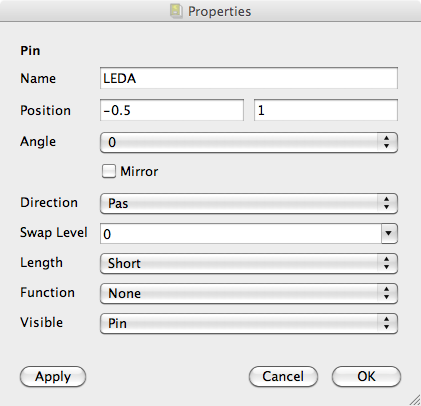
\includegraphics[bb=0 0 421 406, clip, scale=1.0]{pin_property.png}}
	\caption{Диалоговое окно ''Properties'' вывода}
	\label{img:pinProperty}
\end{figure}
Для того, чтобы обозначить вывод схемотического изображения, нужно, используя инструмент
''Pin'' разместить ввывод в нужном месте изображения.


После размещеня всех выводов символа необходимо произвести настройку их свойств.
Для настройки свойств выводов в системе Eagle используется диалоговое окно
''Properties'' (рис. \ref{img:pinProperty}).


Диалог "Pin properties'' системы Eagle позволяет настраивать следующие свойства выводов:

\point{Direction} -- задаёт логическое направление сигнала. Корректное задание этого свойства
важно для правильного прохождения правил электрической проверки (ERC) и автоматического
подключения выводов питания. Свойству Diction может быть назначено одно из следующих
значений:
\begin{itemize}
	\item{} NC  -- вывод не подключён;
	\item{} In  -- вход;
	\item{} Out -- вывод (двухтактный выход);
	\item{} I/O -- двунаправленный вход-выход;
	\item{} OC -- выход с открытым коллектором или открытым стоком;
	\item{} Hiz  -- высокоимпедансный выход (т.е. с тремя состояниями);
	\item{} Pas -- пассивный вывод (используется для резисторов, конденсаторов и т.д.);
	\item{} Pwr -- вход питания ($V_{cc}$, $Gnd$, $V_{ss}$, $V_{dd}$ и т.д.);
	\item{} Sup -- выход питания общего назначения (символ земли, общий провод).
\end{itemize}
При наличии Pwr выхода у символа и если соответствуюзий Sup выход присутствует на схеме,
то подключение этих линий происходит автоматически.


\point{Function} -- задаёт графическое обозначение функции вывода. Может принимать
следующие занчения:
\begin{itemize}
	\item{} None --- нет специальной функции;
	\item{} Dot --- к выводу добавляется изображение инвертирующего символа;
	\item{} Clk --- к выводу добавляется изображение тактирующего сигнала;
	\item{} DotClk --- к выводу добавляются изображения тактирующего сигнала и символ
		инвертированного сигнала.
\end{itemize}


\point{Length} -- задаёт длину вывода. Может принимать следующие значения:
\begin{itemize}
	\item{} Point --- вывод отображается в виде точки, без возможности подключения
		к нему, так же не выводиться его имя;
	\item{} Short  --- длина изображения вывода составит 0.1 дюйма;
	\item{} Middle  --- длина изображения вывода составит 0.2 дюйма;
	\item{} Long --- длина изображения составить 0.3 дюйма.
\end{itemize}

\point{Visible} -- этот параметр определяет,-- будет ли отображаться имя вывода на схеме
или печатной плате. Может принимать одно из следующих значений:
\begin{itemize}
	\item{} Off  --- имя вывода не отображается;
	\item{} Pad  --- имя вывода отображается только на печатной плате;
	\item{} Pin --- имя вывода отображается только на принципиальной схеме;
	\item{} Both --- имя вывода отображается во всех случаях.
\end{itemize}

\point{Swaplevel} -- принимает значение от 0 до 255. Значение 0 обозначает, что вывод не может быть
переставлен местами с другим выводом. Задание другого значения обозначает что вывод может
быть переставлен местами с другими выводами того же символа, обладающими тем же уровнем
SwapLevel.

После задания необходимых свойст всем выводам схемы, можно, используя команду
''DESCRIPTION'', задать текстовое описание символа, после чего необходимо произвести сохранение
библиотеки.

\subsubsection{Создание посадочного места ''LCD Rev.B''}
\begin{par}
Для создания посадочного места необходимо использовать команду
''Pa\-cka\-ge'' меню ''Library''.
В результате работы этой команды на экран будет выведено диалоговое окно,
в котором нужно ввести наименование посадочного места, после чего
выполнить сохранение библиотеки.
\end{par}
\begin{figure}[h]
	\center{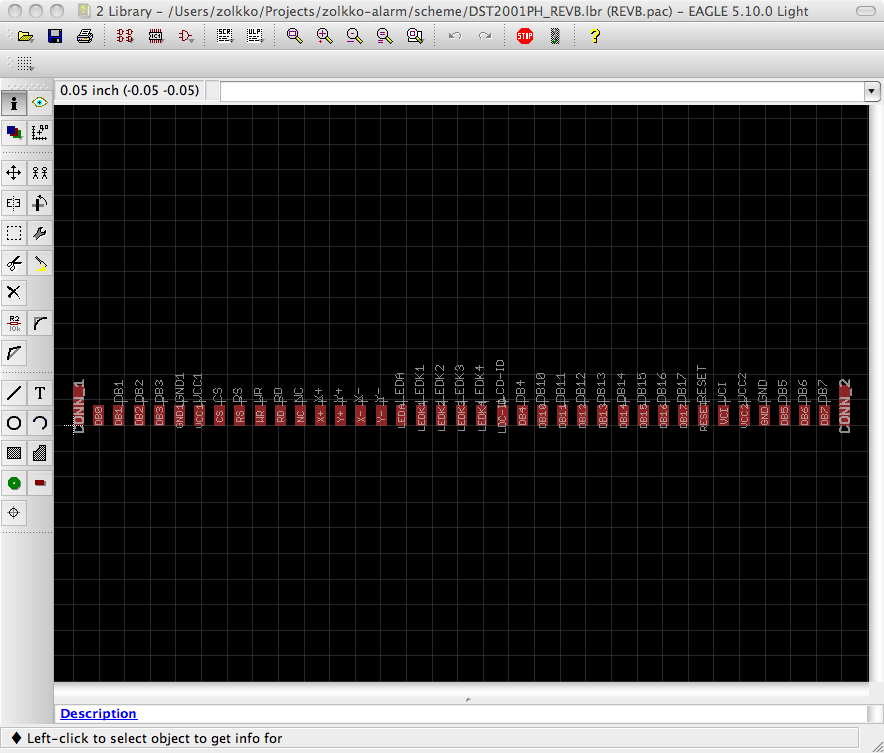
\includegraphics[bb=0 0 884 753, clip, scale=0.5]{package.png}}
	\caption{Окно редактора посадочных мест системы Eagle}
	\label{img:package}
\end{figure}

\begin{par}
По аналогии с редактором символов, в редакторе посадочных мест (рис. \ref{img:package})
необходимо ввести графическое изображение создаваемого посадочного места,
используя инструменты Wire, Rect, Circle и Polygon. 
Контактные плащадки необходимо создавать, используя инструменты ''Surface mount pad'' и ''Pad''.
После чего каждой контактной площадке нужно задать имя. Для этого нужно вызвать диалоговое
окно ''свойства'' (рис. \ref{img:padProperty})  и ввести наимение в поле ''Name''.
\end{par}
\begin{figure}[h]
	\center{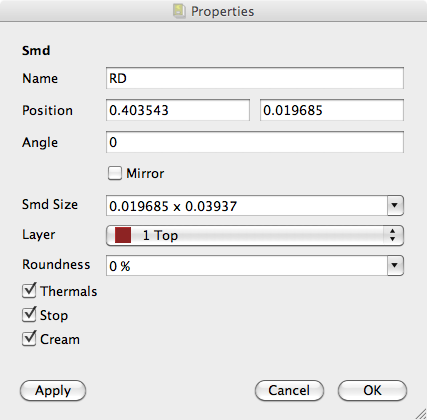
\includegraphics[bb=0 0 421 406, clip, scale=1.0]{pad_property.png}}
	\caption{Диалоговое окно ''Properties'' контактной площадки}
	\label{img:padProperty}
\end{figure}

Размеры самого устройства необходимо задавать на специальном, для этого отведённом, слое.
Обычно для этих целей используется ''tDoc'' слой. Переключившись на него, необходимо, используя
инструменты рисования, задать контуры самого устройства. Прорисовка таких ''физческих'' слоёв
важна для  оптического контроля пересечения или слишком близкого расположения корпусов
устройств на печатной плате.

После завершения формирования посадочного места, можно задать его текстовое описание,
воспользовавшись командой ''DESCRIPTION''.

\subsubsection{Создание устройства ''DST2001PH Rev.B''}
\begin{par}
Последним этапом формирования нового компонента -- является создание ''устройства''.
Устройства (''Device'') в системе Eagle позволяют создавать ассоциацию символа к
одному или нескольким посадочным местам.

Для создания устройства нужно вызвать команду ''Device'', что приводит к отображению на экране
окна редактирования устройств (рис. \ref{img:device}).
\end{par}
\begin{figure}[h]
	\center{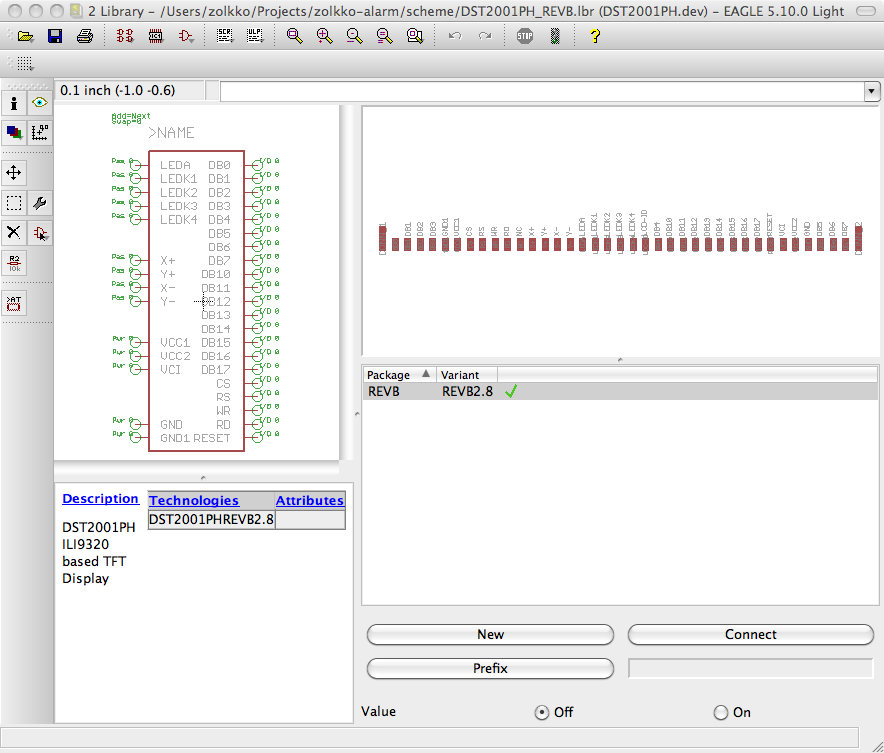
\includegraphics[bb=0 0 884 753, clip, scale=0.5]{device.png}}
	\caption{Окно редактора устройств системы Eagle}
	\label{img:device}
\end{figure}

В окне редактора устройств нужно, используя инструмент ''Add parts'', разместить в области
редактирования нужный символ. А нажатие кнопки ''New'' области задания посадочного места,
позволит проассоциировать с данным символом нужное посадочное место.

В случае, если одному символу нужно поставить в соответствие несколько корпусов, то каждому
вновь добавляемому в список корпусу нужно задавать имя. Обычно для интегральных
микросхем в качестве такого имени используют постфиксы, используемые для обозначения
различных видов корпусов одной и той же микросхемы, принятые у производителя. Однако,
так как устройство DST2001PH\_REV.B существует только в одном корпусе, поле названия варианта
можно оставить не заполненным.

\begin{figure}[h]
	\center{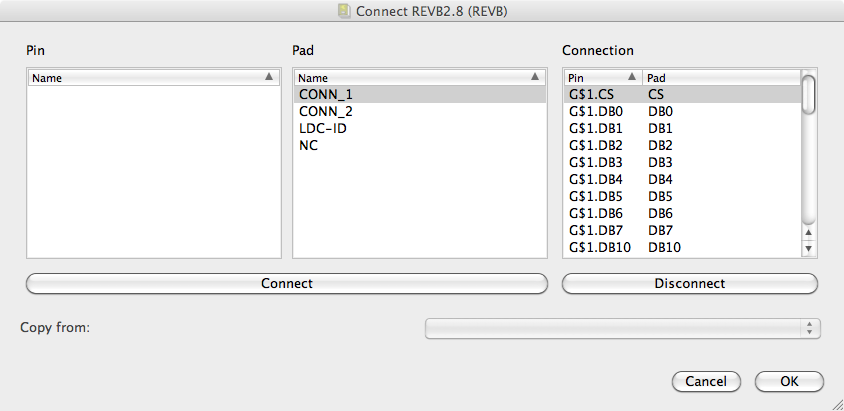
\includegraphics[bb=0 0 844 411, clip, scale=0.5]{dev_connect.png}}
	\caption{Окно редактора устройств системы Eagle}
	\label{img:devConnect}
\end{figure}
Важным моментом в процессе создания устройства является проведение ассоциации выводов
символа с контактными площадками посадочного места. Эта операция осуществляется
в диалоговом окне ''Connect'' (рис. \ref{img:devConnect}), вызываемом при нажатии на кнопку ''Connect''.

\subsubsection{Перечень сформированных символов, посадочных мест и устройств}










